\section{Mining Next Generation}
\label{sect:mining}

Traditionally blocks in a blockchain contain an ordered list of transactions
combined with a cryptographic hash ---Blake2b \cite{aumasson2013blake2} in our
case--- of the previous block \cite{whatisablockchain,raikwar2019sok} and mining
is the act of creating such blocks. Transactions are only added with the
creation of a new block which. In \cite{Eyal:2016:BSB:2930611.2930615}
Ittay et al. propose to decouple the leader election from inclusion of
transactions in blocks for scalability purposes. Their scheme dubbed
\enquote{Bitcoin-NG} is what we adopted using Cuckoo Cycle for proof-of-work.

% Chaining of hashes prevents that blocks can be tampered with. If a block
%changes with even one bit, the hash of the block will change.
%The changed block's successor will then contain the hash of a non-existing
%block. Thus, an attacker modifying a transaction in a block will also have to
%modify all consecutive blocks. Since the hashes also have to satisfy a
%difficulty requirement, which requires a non-trivial amount of work, rewriting
%a block in the history of the chain is assumed to require more computational
%resources than available to an attacker.

\subsubsection{Cuckoo Cycle PoW}

\textit{Cuckoo Cycle} \cite{Tromp2015CuckooCA}, a graph-theoretic problem of
finding cycles in a graph, is used for proof-of-work puzzles. Finding solutions
to this problem is memory bound, meaning that runtime is constrained by memory
latency of accessing nodes of the graph. Cuckoo cycle was chosen because memory
latency is believed to not allow as big performance gains from specialised
integrated circuits (ASICs) versus general purpose hardware. Verifying the
validity of a solution is also trivial, meaning that validating a block has
less overhead.

Solving a cuckoo cycle instance requires finding a fixed length cycle in a
bipartite graph of $2^N$ edges and $2^M$ nodes. The ratio of $\frac{M}{N}$,
$\frac{1}{2}$ by default, is one of the parameters to control the hardness of
the problem. Edges are represented as $N$ bit strings.
As of December 2019, \aet\ requires cycles of length 42 and the 30 bit edges.

\subsubsection{Difficulty}

Adaptable difficulty allows us to control the expected time it takes to find
a solution and thus a new valid block. To allow more fine-grained control over
the difficulty of the proof-of-work, the final step after a solution to the
graph problem has been found is to hash it.
The hash is then compared to a difficulty target, which is adjusted with
each new block. If output of the hash function and the difficulty target are
interpreted as numbers, then in order to have a valid proof-of-work solution,
the hash needs to be smaller than the target difficulty.

The difficulty for each block is deterministically computed based on timestamps
of the last 17 blocks. This timestamp is unreliable, since the nodes have no
synchronized clocks. However, the timestamp may not precede the timestamp of a
previous block. A block submitted with difficulty not meeting the target
specified in the previous block will be ignored by honest nodes.
Likewise, if a miner presents the wrong target difficulty for the next block,
this block will be discarded.

\subsubsection{Forks}

Whenever there are two or more blocks produced with the same parent block, we
speak of a \textit{fork}. This can happen for a variety of reasons, accidental
or intended. Forks can last for multiple blocks with miners working on separate
branches.
A defining feature of every blockchain is the \textit{fork choice rule}. It
tells honest nodes which branch to choose in case of a fork. For \aet nodes,
the rule is to prefer the longest branch use work committed to it, as measured
via the difficulty, as tiebreaker.

A different kind of fork can be caused whenever nodes run different software
and disagree about the rules of what constitutes a valid block. In this case
manual intervention by node operators might be required.

%\subsubsection{Finality}

%The most important metric for a majority of blockchain users is the latency
%between submitting a transaction and the time by which there is enough
%certainty to consider this transaction confirmed, i.e. final. How to
%quantify this metric is still an understudied topic but beyond the scope of
%this paper.
%The most widely used metric nowadays, although certainly not the best, is the
%number of blocks following the block which included the transaction in
%question.
%This metric is used with the assumption that with each successive block the
%probability of a previously unknown, but longer, branch with more work
%committed, showing up, gets lower. Such an unknown branch could be problematic
%since it might include different transaction and invalidate a previously
%thought to be valid transaction.
%The logic for this follows from the above fork choice rule and the lack of a
%way of assessing the actual mining power available to all network
%participants.

\subsection{Bitcoin-NG}

Where in Bitcoin or Ethereum each block filled with transactions requires
a proof-of-work solution, a miner in \aet\ has to find one proof-of-work
solution and can then create multiple blocks with transactions until the next
miner finds an admissible proof-of-work solution. This scheme was proposed by
Ittay et al. \cite{Eyal:2016:BSB:2930611.2930615} under the name \enquote{Bitcoin-NG}.

\subsubsection{Key- and micro-blocks}

Bitcoin-NG requires two different kinds of blocks. One kind, called
\textit{key-block}, to elect the miner, or \textit{leader}, who is allowed to
include transactions on chain, and \textit{micro-blocks} containing
transactions. Every new key-block starts a new epoch---or \textit{generation}
in the \aet\ context.

The key-blocks contain the hash of a previous micro-block as well as the hash
of the previous key-block.
Micro-blocks are being created in rapid succession making it likely that any
given new key-block does not include the hash of the latest micro-block
produced by the previous round leader.
This is called a micro-fork. (cf.\ red micro-block in Fig.\
\ref{ng-mining}). The transactions of the discarded micro-blocks are put back
in the transaction pool and taken care of by the next leader. Since they have
been seen in a micro-block before, they will very likely be valid in
future micro-block as well.

In practice, miners are allowed to publish a micro-block every three seconds
and the computational complexity---associated with every transaction and
measured in gas---is limited per block. These limits are put in place to avoid
miners flooding the network.

To give miners an incentive to work on top of the newest micro-block,
transaction fees are divided by giving 40\% to the leader producing a
micro-block and 60\% to the miner of next key-block after that
micro-block\footnote{Note that if miners
  were to only mine key-blocks, there would be no transactions on the
  chain at all.}.

\begin{figure}
   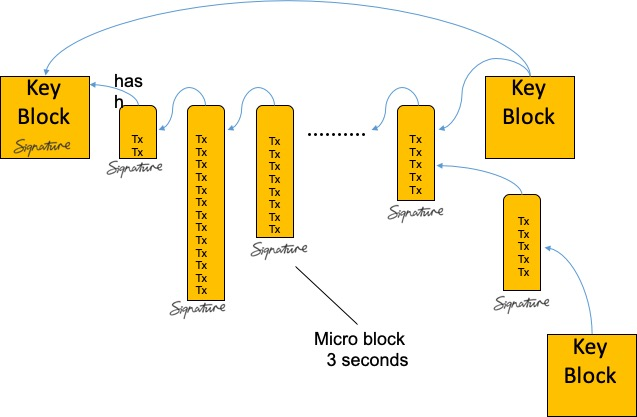
\includegraphics[scale=0.3]{keymicro.jpg}
   \caption{Next generation consensus}
   \label{ng-mining}
\end{figure}

\subsubsection{Fraudulent leaders}

There is only one leader per generation creating micro-blocks. Each key-block
includes the public key of the new leader and consecutive micro-blocks are
only valid if signed with the associated private key. This protects
against third parties trying to post micro-blocks.

A malicious leader, however, could construct forks either by forking directly
from the key-block, or by forking on a micro-block. This could be done to
disrupt the network or to perform double spend attacks. A malicious miner could
also try to produce more micro-blocks than entitled to by fiddling with the
micro-block creation timestamp.

In order to mitigate the risk of a leader forking its own sequence,
there is a mechanism in place to detect and report this by submitting
a Proof-of-Fraud. This is submitted in the next
generation. The leader is punished by not receiving a block reward and
in order to make that possible, block rewards are not immediately paid out but
kept for the duration of 180 blocks.

\subsubsection{Divide and conquer}

Each transaction is a binary of a certain size. Internally both size
and computation are expressed in gas and there is a maximum amount of
gas per micro-block that allows for maximally 300 KB per micro-block.
Thus, an additional advantage of the introduction of micro-blocks is that
instead of a huge block with 180,000 transactions in 3 minutes, we can create
60
reasonably sized micro-blocks of maximally 300 KB  in the same 3
minutes. This has several advantages for network latency and
smaller blocks are easier and faster to gossip through the
network. Moreover, if it takes longer to compute the next key-block we
are not bound to a maximum block size, because we generate new
micro-blocks as long as no key-block has been found.